The previous chapter introduced a data augmentation method for manipulation. We used this method to learn reliability for dual-arm rope manipulation in from real world data. The dynamics model used in these experiments was also trained on real world data, in a separate phase that was designed to ensure no contact between the rope and the environment. This extra step was time-consuming and hand-designed, and attempts to use free-space dynamics pretrained in simulation failed because the simulation and the real world rope dynamics were too different.

This chapter address this problem, by proposing a novel dynamics adaptation method. Our key insight is that a free-space data from simulation is far more similar to free-space data from the real world than it is to non-free-space data from the real world. More generally, the problem we address is to adapt a dynamics model from a source environment to a target environment, where the source and target dynamics are similar in some regions but different in others. Our proposed adaptation method focuses adaptation on data where the dynamics are similar, which we show leads to more accurate dynamics for planning and good estimates of the dynamics model's reliability. Ultimately, we use this method to simultaneously adapt a dynamics model learned in simulation and learn reliability -- all online and in the real world.

\section{Introduction} \label{ICRA:sec:intro}

 Learning dynamics models for manipulation is an increasingly popular paradigm, in part because learned models can be repeatedly improved using autonomously collected real-world data. However, fine-tuning an initial dynamics model on new data can perform poorly when the data contains complex dynamics on which the dynamics model was not initially trained. For example, suppose we want to manipulate a rope amongst clutter, and we have a dynamics model trained on free-space motions in simulation. Free-space transitions in the real world are fairly similar to the free-space in simulation, but transitions where the rope deforms on objects in the scene are very different from anything seen in simulation. We call these transitions \emph{distracting}, because they are hard to learn from a few examples, and because they make it harder to adapt accurately to the free space dynamics. More generally, transitions from regions of dissimilar dynamics can inhibit effective transfer to regions of similar dynamics. This problem is similar to ``cleaning'' data in machine learning \cite{mislabeled99,filtering21,anomoly22}. For dynamics learning, defining what ``clean'' means can be difficult, and has not been studied extensively. Instead, the dominant paradigm is simply to train on all the collected data.

However, training on all the data can fail because real world datasets for learning dynamics are often too small to learn generalized models over the entire state-action space. In our experiments, we show that simply fine-tuning on all the data can yield a model that is not accurate enough for planning. If the task can be completed while remaining in regions where dynamics are similar, then it can be worth trading accuracy in dissimilar regions for accuracy in similar regions.
Our key insight is that, when we are adapting from an initial model, we can leverage the initial model to achieve significantly lower prediction error by focusing on transitions where the source and target dynamics are the most similar. The idea that transfer is easier when the source and target data are similar is well-supported in the transfer learning literature ~\cite{sorocky2020experience,bocsi2013alignment}.

\begin{figure}
    \centering
    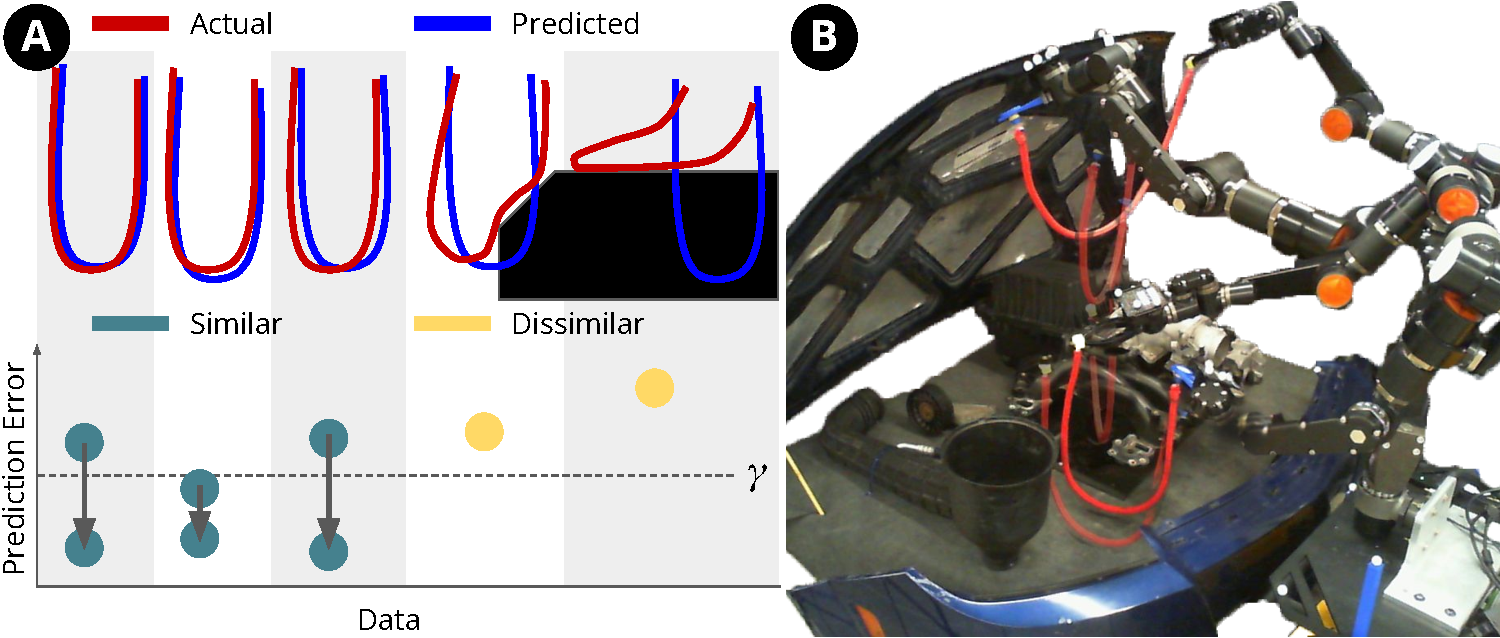
\includegraphics[width=1\linewidth]{Chap4/images/title_figure.pdf}
    \caption{
    (A) An illustration of how our adaptation method focuses on regions where the source and target dynamics are similar. When focusing adaption on free-space dynamics, the prediction errors decrease for other free-space data (similar), do not decrease for collision dynamics (dissimilar).
    (B) A mock-up of a car engine bay. The robot must move the rope and place it under the engine without snagging it to set up for lifting the engine. We use our proposed adaptation method to improve success rate during online learning for this task.}
    \label{ICRA:fig:real_robot_setup}
\end{figure}

To implement this strategy, we propose an adaptation method which minimizes prediction error in regions where the source and target dynamics are similar. The proposed method minimizes prediction error in these regions by fine-tuning on an initially small set of data from these regions, and growing that subset over the course of training. This is done with a loss function inspired by curriculum-learning that weighs transitions according to their prediction error, assigning higher weight to low-error transitions. Under the assumption that there are paths to the goal where the source and target dynamics are similar, this adaptation method can be used to achieve high task success in the target environment.

The first contribution of this chapter is a method for adapting dynamics models to datasets which contain distracting transitions. We demonstrate the proposed method is successful in filtering out distracting data and that the resulting trained model is more accurate in the regions of state-action space where the source and target dynamics are similar. The second contribution is a data-efficient online-learning method that pairs our adaptation method with prior work on planning with unreliable dynamics models \cite{UnreliableMitrano2021,MDEs22}. We call our combined method for online learning \FOCUS{}. \FOCUS{} achieves higher success rates in the low-data regime because the adapted dynamics are more accurate, which leads to finding more reliable plans.
\section{Problem Statement} \label{ICRA:sec:problem_statement}

The problem addressed in this chapter is to adapt a dynamics model trained in a source environment to data collected in a target environment, where the source and target environments have dynamics which are similar in some regions of the state-action space, but different in others. Furthermore, we consider the case where data collection is done by planning and executing paths to goals in the target environment using the learned dynamics model.

To formalize this, first consider the standard dynamics learning problem with a dataset $\dataset$ of transitions of states, actions, and next states $\transition$. We also assume a distance function $\distf{\state_1}{\state_2}$ that returns a scalar is given. The true dynamics are $\state'=\dynamics(\state,\action)$, and the learned dynamics are $\pred{\state}'=\learnedDynamics(\state,\action)$. We propose defining the source and target environment dynamics as similar for a transition if $\distf{\sourceDynamics(\state,\action)}{\targetDynamics(\state,\action)} < \softFilteringThrehsold$. The threshold $\softFilteringThrehsold$ should be small enough that it excludes distracting transitions, but large enough to include as much data from the target environment as possible. Let $\DST$ be the set of transitions from the target environment where this similarity condition holds.

In order to minimize the amount of data needed for adaptation to generalize, we aim to adapt the dynamics only to transitions from regions where this similarity condition holds ($\DST$). However, we also care about successfully completing the task, and therefore we also assume there are paths $\traj$ to the goal $\state^T\in\goal$ within the regions of similar dynamics $(\state^t,\action^t,\state^{t+1}) \in \DST $.

While the ultimate objective of adaptation should be to maximize task success in the target environment, an important condition for task success is minimizing prediction error on $\DST$. If the goal is reachable within $\DST$ (as we assume), the prediction error on $\DST$ is small (our objective), and our motion planner is constrained to stay in $\DST$, then we can also expect high task success. Next, we discuss how our adaptation method minimizes error on $\DST$, followed by how we can achieve high task success by additionally constraining a motion planner to $\DST$.

\begin{figure}
    \centering
    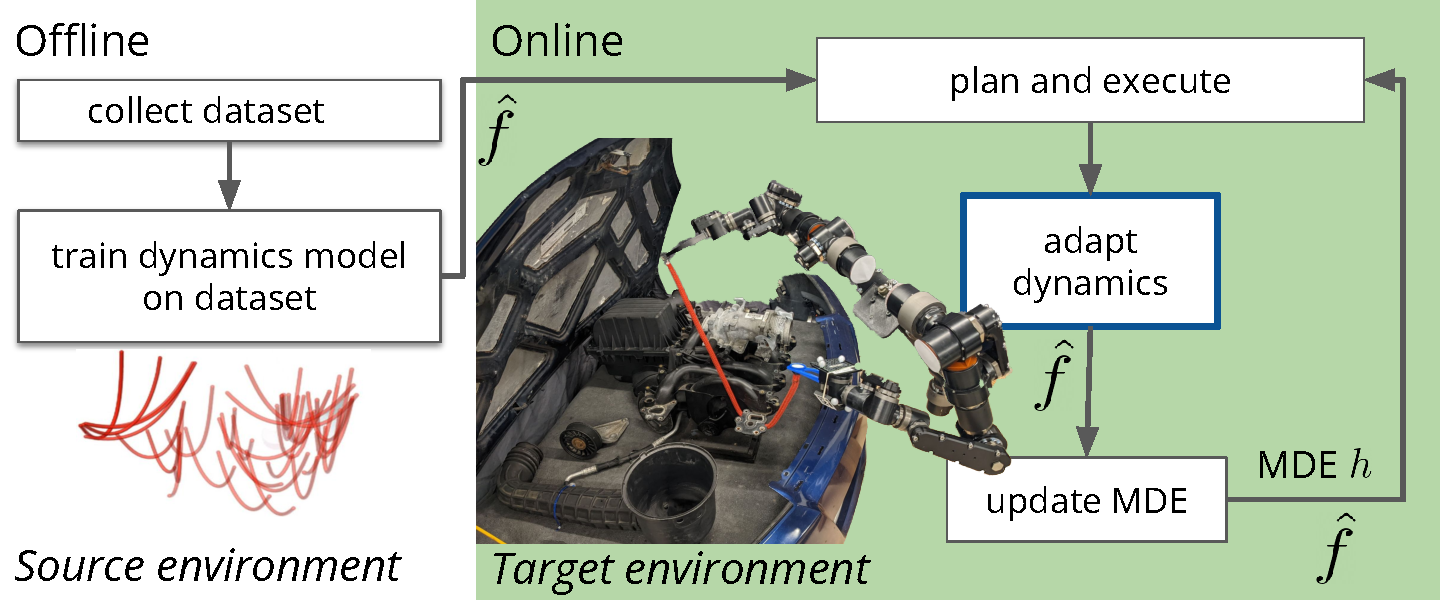
\includegraphics[width=1\linewidth]{Chap4/images/overview_diagram.pdf}
    \caption{Block diagram showing the steps of our full online adaptation method. A dynamics model is initialized offline in the source environment (left), then adapted online in the target environment.}
    \label{ICRA:fig:diagram}
\end{figure}

\section{Methods} \label{ICRA:sec:methods}

\subsection{Adapting the Dynamics} \label{ICRA:sec:adaptation}

At a high level, our method minimizes prediction error on $\DST$ by dynamically weighing the training data $\dataset$ such that transitions that are likely to be in $\DST$ are given weights near 1 and transitions unlikely to be in $\DST$ are given weights near 0. Given a transition from our training data $\transition\in\dataset$, we cannot directly evaluate whether that transition is in $\DST$, since that would require knowing the true dynamics $\targetDynamics$. However, since the initial dynamics, denoted $\learnedDynamics_0$, is assumed to accurately fit the source dynamics, it is likely that transitions with low prediction error under the initial dynamics $\distf{\learnedDynamics_0(\state,\action)}{\state'\big} < \softFilteringThrehsold$ are in $\DST$. By training on transitions with initially low error, we expect the prediction error on other transitions which belong to $\DST$ to also decrease. This slowly brings more and more transitions to have prediction errors below $\softFilteringThrehsold$. On the other hand, the prediction error is unlikely to decrease for transitions not in $\DST$, because they are dissimilar to the transitions with low initial error. Thus, at each step $j$ of training, we assign each transition a weight as a function of the prediction error $||\pred{\state}'-\state'||^2$, and multiply this weight by the loss. The full loss is shown in Equation \eqref{ICRA:eq:adaptation_loss}.

\begin{equation}
    \label{ICRA:eq:adaptation_loss}
    \begin{split}
    \mathcal{L}_\dynamics &= \frac{1}{T}\sum_{t=1}^T\Big(\dynamicsErrort w^t\Big) \\
    w^t &= 1 - \sigma\big(\phi(\globalStep)(\dynamicsErrort - \softFilteringThrehsold)\big)
    \end{split}
\end{equation}

$\sigma$ is the sigmoid function. When $\globalStep$ is large, the boundary is almost hard, and transitions with error below $\softFilteringThrehsold$ have weight near 1 and transitions with error above have weight near 0. When $\globalStep$ is small, the boundary is soft, and the weights vary less. The term $\phi(\globalStep)$ controls the rate of change of hardness. We use $\phi(j)=0.5j$ in our experiments. We found that allowing the weighting to be soft during early training steps improves the stability in the case where few or no transitions have error below $\softFilteringThrehsold$ at the beginning of training. The parameter $\softFilteringThrehsold$ can be chosen based on either the maximum error that can be corrected by a low-level controller, or based on the distribution of error on a validation set from the source environment (e.g the 97th percentile).

\subsection{Online Learning}

\begin{figure}
    \centering
    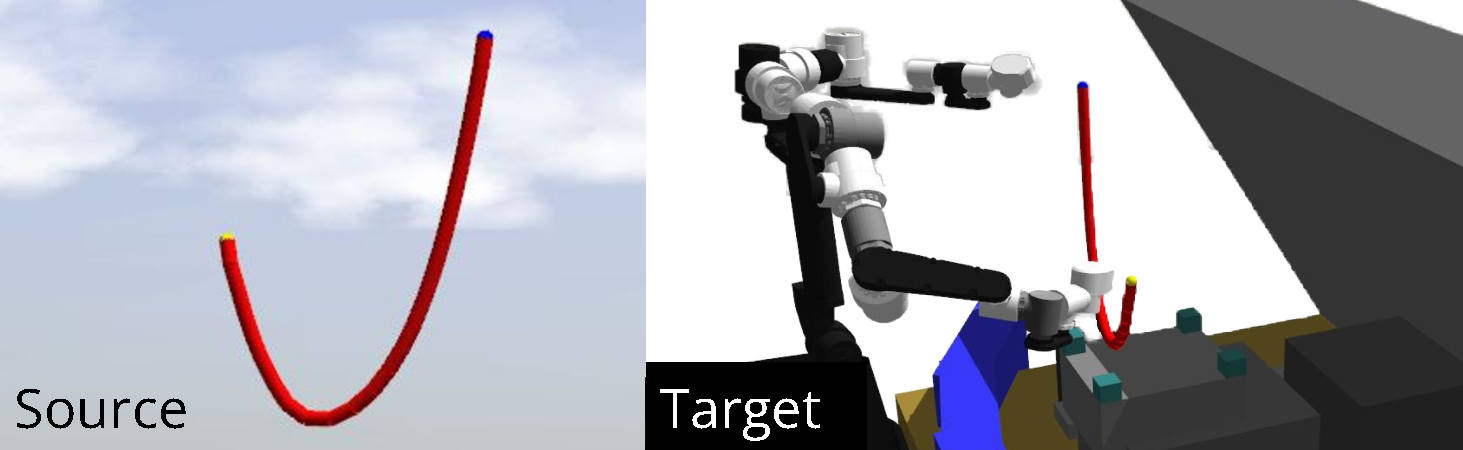
\includegraphics[width=\linewidth]{Chap4/images/sim_rope_envs.pdf}
    \caption{Source environment for bimanual rope manipulation (left) and simulated target environment (right) where there is a robot, obstacles, and the rope damping and stiffness are changed.}
    \label{ICRA:fig:sim_rope_envs}
\end{figure}

\begin{figure}
    \centering
    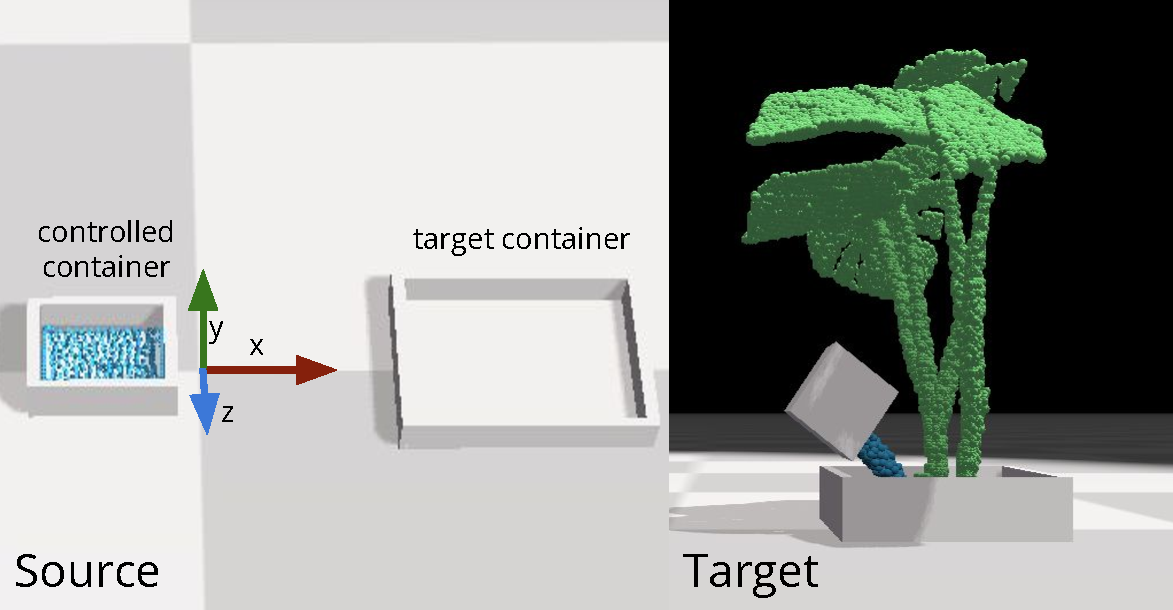
\includegraphics[width=0.7\linewidth]{Chap4/images/sim_water_envs.pdf}
    \caption{Source environment for plant watering (left) and target environment (right) where there is an additional plant, and the viscosity is tripled.}
    \label{ICRA:fig:waterscene}
\end{figure}

In this section, we describe how the proposed adaptation method can be combined with prior work on planning with unreliable dynamics to achieve data-efficient online adaptation of dynamics models. A block diagram of the full method, which we call \FOCUS{}, is shown in Figure \ref{ICRA:fig:diagram}. \FOCUS{} consists of an offline phase and an online phase. In the offline phase, we train a dynamics model using data from the source environment, which in our experiments is a simple simulation. We use random actions to collect a diverse set of data and standard techniques for training the neural network dynamics model \cite{UnreliableMitrano2021}.

In the online phase, we adapt the learned dynamics model to the target environment (e.g. the real world). This process alternates between (1) collecting new data in the target environment by planning and executing, (2) fine-tuning the dynamics, and (3) fine-tuning the model deviation estimator (MDE). We now explain the data collection and MDE fine-tuning steps.

\subsubsection{Planning and Execution for Data Collection}

We use a kinodynamic RRT planner where nodes are propagated using the learned dynamics model. Since the learned dynamics are adapting to only $\DST$ and are not accurate everywhere, we additionally constrain the planner to stay in $\DST$. Since $\DST$ is not known \textit{a priori}, we train another neural network, called a model deviation estimator (MDE)~\cite{MDEs22, UnreliableDale2019, UnreliableMitrano2021}, to predict the error of the dynamics model (more details in Section \ref{ICRA:sec:fine_tuning_mde}). In addition to producing more robust plans, planning with MDEs has the additional benefit of focusing data collection on $\DST$. By collecting more data where the source and target dynamics are close, a larger fraction of $\dataset$ is likely to be in $\DST$, and therefore the adaptation procedure has more data from which to learn.

We use the MDE in planning as a constraint checker. If the dynamics error predicted by the MDE is below a threshold $\dmax$, then we add it to the planning tree. We also randomly accept transitions with high predicted dynamics error with low probability (0.01), so that the planner will occasionally return paths with exploratory actions (we call these \textit{random-accepts}). These exploratory actions are essential for training the MDE, since they can correct over-estimation of model error from the MDE. The threshold $\dmax$ for allowable error is similar to $\softFilteringThrehsold$, but may be set higher or lower to control the exploration/exploitation tradeoff.

The robot uses the planner to attempt the task, and repeatedly plans and executes open-loop until a timeout or the goal is reached. If no plan is found that reaches the goal, the plan which gets closest to the goal is executed. This repeated planning and execution is called one episode. After some fixed number of episodes (e.g. 10) we fine tune the dynamics and the MDE using all data collected so far during the online phase.

\subsubsection{Fine-tune MDE}
\label{ICRA:sec:fine_tuning_mde}

The MDE is used to constrain planning to regions where the dynamics model is predicted to be accurate, which has two benefits. First, it helps bias data collection to contain transitions from $\DST$. Second, it makes reaching the goal more likely since it avoids plans that do not match to the true dynamics. The MDE $\pred{\mdeError}=\MDE(\env,\state,\action,\pred{\state}')$ is a convolutional neural network which takes as input the environment, state, action, and next predicted state, and predicts the error of the dynamics model $\pred{\mdeError}$. We represent the environment $\env$ as a voxelgrid of the scene. The ground truth error used for training is the error between the true observed state and the state predicted by the learned dynamics: $d=\distf{\pred{\state}'}{\state'}$. The loss function is shown in Equation \eqref{ICRA:eq:mde_loss}. Intuitively, the MDE should be easier to learn with fewer data than learning the dynamics accurately everywhere, since the MDE need only predict the magnitude of the error as opposed to the full state vector \cite{UnreliableMitrano2021}.

\begin{equation}
    \label{ICRA:eq:mde_loss}
    \mathcal{L}_{\MDE} = ||\pred{\mdeError} - \mdeError||^2e^{-{\kMDE \mdeError}}
\end{equation}

$\kMDE$ is a hyperparameter that reduces the need to predict high dynamics errors with high accuracy. We set $\kMDE=10$.

\section{Results} \label{ICRA:sec:results}

We begin by describing the two domains for our experiments: bimanual rope manipulation and plant watering. We then validate the claims that (1) our proposed adaptation method achieves lower prediction error in regions of similar dynamics, and (2) that \FOCUS{} achieves higher success rates more quickly in the online adaptation setting compared to baselines which train on all data equally.

\subsection{Bimanual Rope Manipulation}
\label{ICRA:sec:rope}

\begin{figure*}
    \centering
    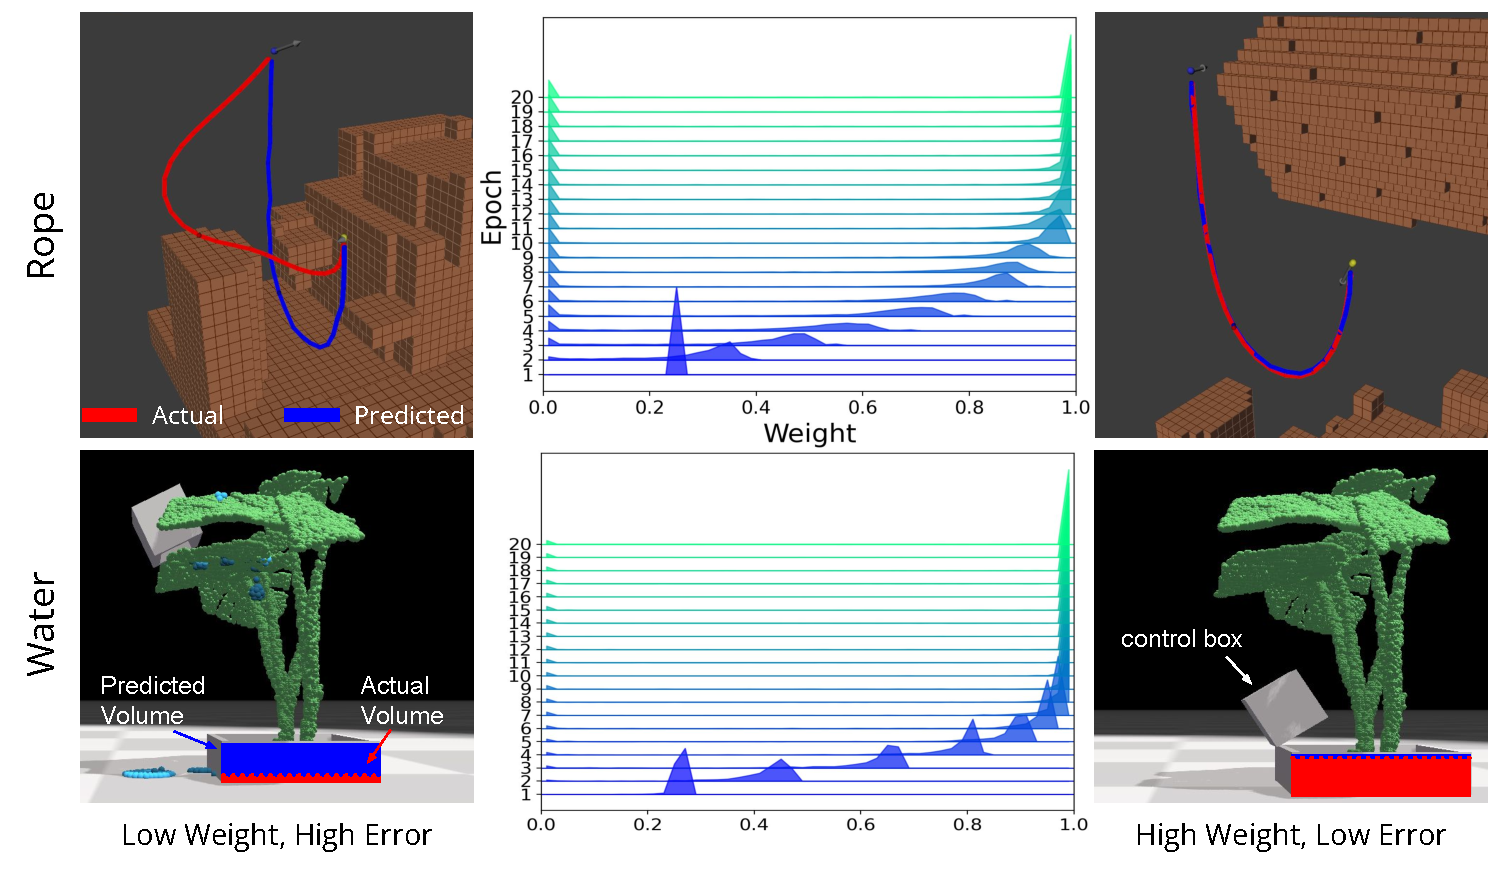
\includegraphics[width=\linewidth]{Chap4/images/data_weight_distribution_figure.pdf}
    \caption{(center) Histograms showing weights assigned to the data according to Equation \eqref{ICRA:eq:adaptation_loss} during the first 20 epochs of training. A histogram is shown for each epoch, where color varies with epoch, and these histograms are staggered along the y-axis. Initially, the weights vary only slightly across the data, but the distribution becomes strongly bimodal as training progresses. Examples of transitions given weight 0 (left) and weight 1 (right) at the end of training.}
    \label{ICRA:fig:weights}
\end{figure*}

In this task, a 16-DOF dual arm robot is holding two ends of a rope in a scene resembling the engine bay of a car (scene shown in Figures \ref{ICRA:fig:real_robot_setup},\ref{ICRA:fig:sim_rope_envs}). The task mimics putting on lifting straps on the engine, which requires moving the rope through narrow passages and around protrusions. The goal is to place the middle of the rope in a goal region defined as a sphere of radius \SI{0.045}{\meter}. The planner outputs gripper position actions, and a local controller executes the actions while maintaining gripper orientations. The learned dynamics model predicts the state of the rope, represented as 25 points, given the initial rope state and gripper position actions.

In the rope manipulation experiments, the source simulation has no obstacles and the robot is simplified to floating kinematic grippers. We then test adaptation to two different target environments: (1) another simulation which includes the robot and obstacles and has different damping and stiffness parameters for the rope, and (2) the real world. Thus, this tests adaptation to a different rope despite the distracting transitions where the rope deforms on the robot or the obstacles. Gazebo with ODE physics is used for simulation \cite{Gazebo}. For rope manipulation, the set $\DST$ would be the transitions from the target environment where the rope is in free space. We use $\softFilteringThrehsold=0.08$.

\subsection{Plant Watering}
\label{ICRA:sec:water}

The goal in this task, illustrated in Figure~\ref{ICRA:fig:waterscene} is to pour at least 75\% of the initial volume from a controlled container into a target container without spilling more than 5\%. The source environment is a variation from the SoftGym PourWater environment~\cite{lin2020softgym}. The target environment has triple the viscosity, a shorter container, and a plant in the target container. Although the agent can pour from above, that causes the water to splatter, which is more difficult to predict than the free-space pours of the target environment. Additionally, the box can collide with the plant, which is dissimilar to the source dynamics where there are no obstacles. The controlled container can rotate about the z-axis The state space is the 4-DOF $[x,y,z,\theta]$ pose of the controlled container, 3-DOF $[x,y,z]$ pose of the target container, control volume, and target volume. The action space is a target pose $[x_{des}, y_{des}, \theta_{des}]$ which is followed by a proportional controller. For plant watering, the set $\DST$ contains free-space motions and pours, whereas collision with and pouring on the plant is not in $\DST$. We use $\softFilteringThrehsold=0.05$.

\subsection{Validating the Adaptation Method}
\label{ICRA:sec:validating_adaptation}

\begin{figure}
    \centering
    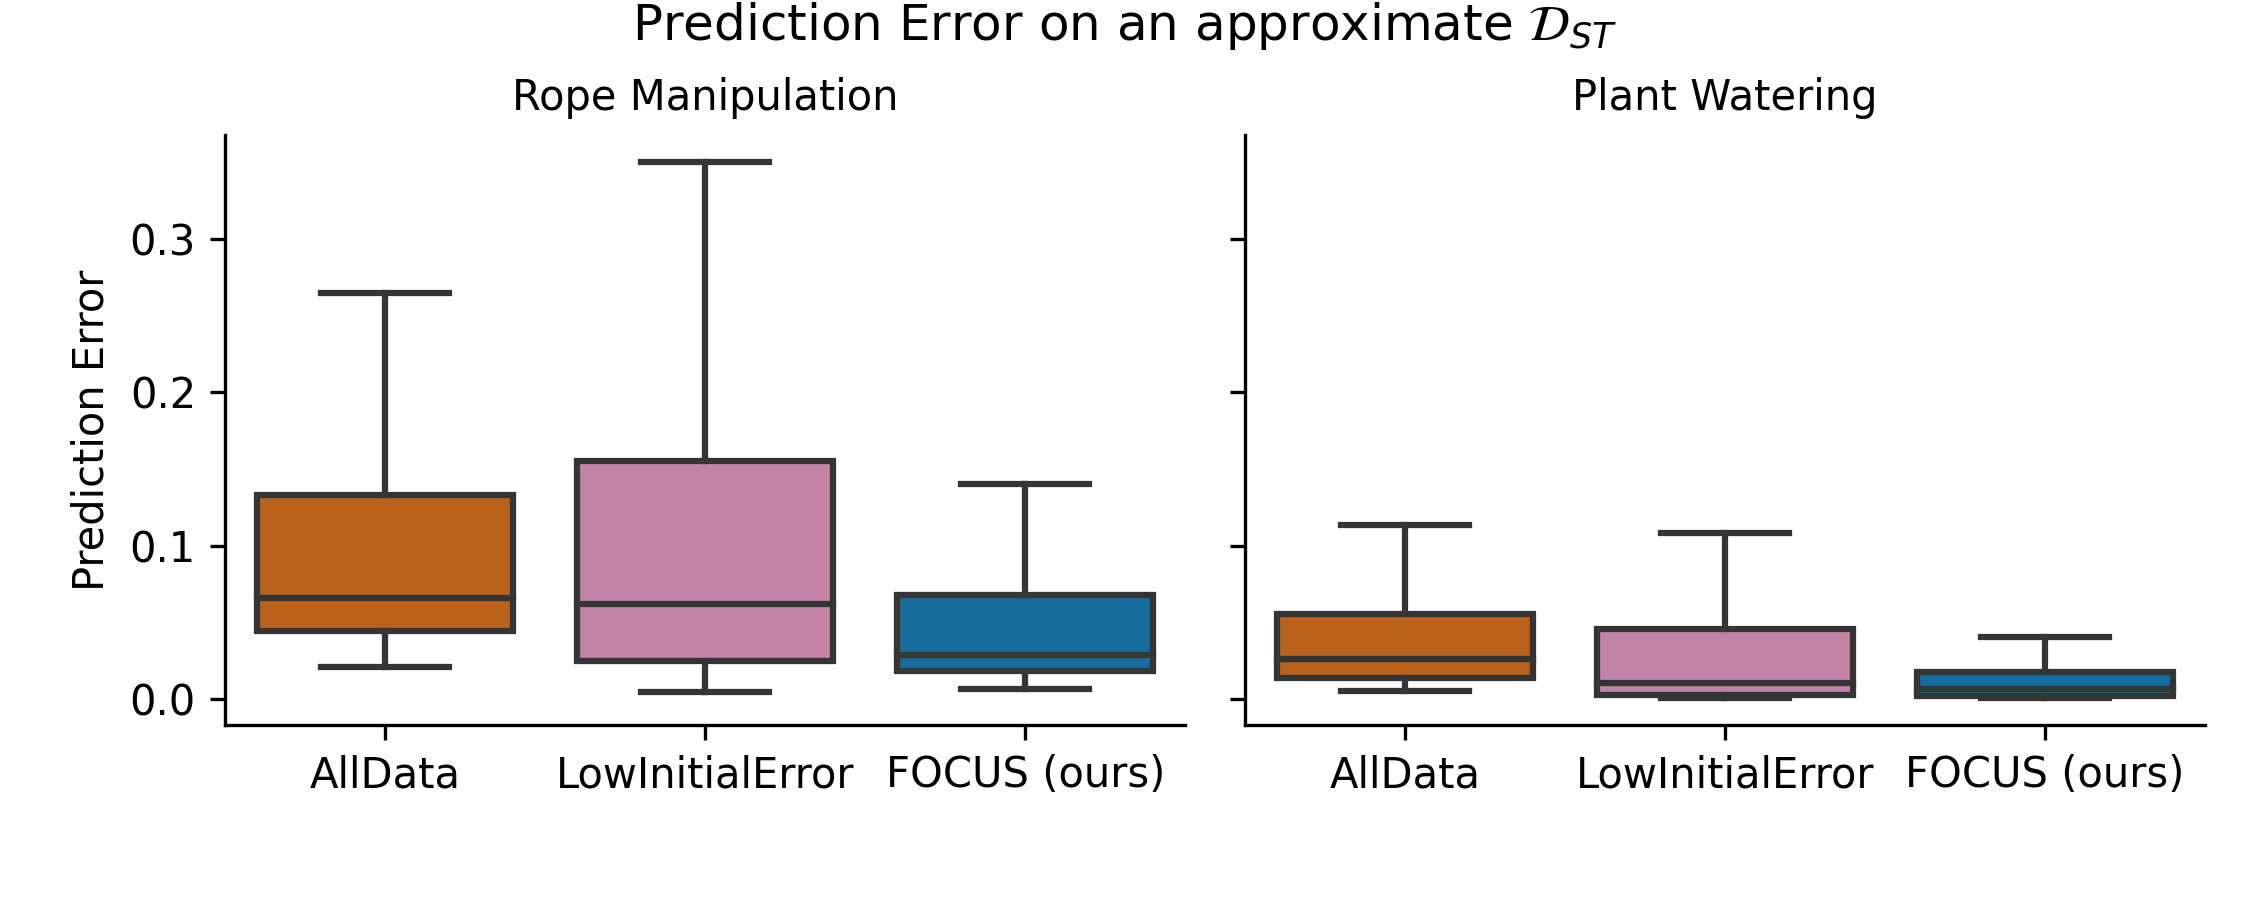
\includegraphics[width=\linewidth]{Chap4/images/known_good_model_error.png}
    \caption{Prediction error for our method versus two baselines, evaluated on a dataset of transitions from regions where the source and target dynamics are similar.}
    \label{ICRA:fig:validating}
\end{figure}

We now evaluate whether the proposed adaptation method achieves lower prediction error on $\DST$. We start by creating validation sets which contain transitions not used for training, and which are known to be in $\DST$. For rope, this means transitions where the rope is in free space. For water, this means transitions which do not collide with or pour over the plant. We evaluate our method and two baselines, all starting from the same pre-trained model and adapting to the same dataset from the target environment. The baseline \textit{AllData} fine-tunes on all transitions with equal weights. The baseline \textit{LowInitialError} uses our weighting function, but computes the weights once using $\learnedDynamics_0$ and does not re-compute them throughout training. Our method uses our proposed loss function (Equation \eqref{ICRA:eq:adaptation_loss}) which re-computes the weights on each batch during training.

For bimanual rope manipulation, the dataset contains 6288 transitions and the validation set contains 792 transitions. For plant watering, the training dataset contains 854 transitions and the validation set contains 130 transitions. The results are visualized in Figure \ref{ICRA:fig:validating}. In both experiments, the error of our method is statistically significantly lower than both baselines ($p<0.0001$).

Figure \ref{ICRA:fig:weights}, demonstrates the intuition behind our adaptation method. In the center, we show histograms over time of the weights assigned to the transitions in the training dataset, for water and for rope. The distribution is initially unimodal since the weighting function when $j=0$ is soft, but as training progresses the distribution rapidly becomes bimodal, where most transitions are given a weight of 1, but some transitions are given a weight of 0. We show examples of these low and high weight transitions on either side. For rope manipulation, we found that the number of the transitions with prediction error below $\gamma$ increases from 52\% at epoch 1 to 80\% at epoch 20, which shows that the subset of data we train on grows. This explains why our method outperforms the \textit{LowInitialError} baseline, since that baseline is not making use of as much of the data as our method does. The presence of transitions with 0 weight (e.g. 20\% for rope at epoch 20) shows that our method is not converging to training on all examples, which does not perform well based on the \textit{AllData} baseline.

\subsection{Online Learning Experiments}
\label{ICRA:sec:online_learning_experiments}

\begin{figure*}
     \centering
     \begin{subfigure}[b]{0.32\textwidth}
         \centering
         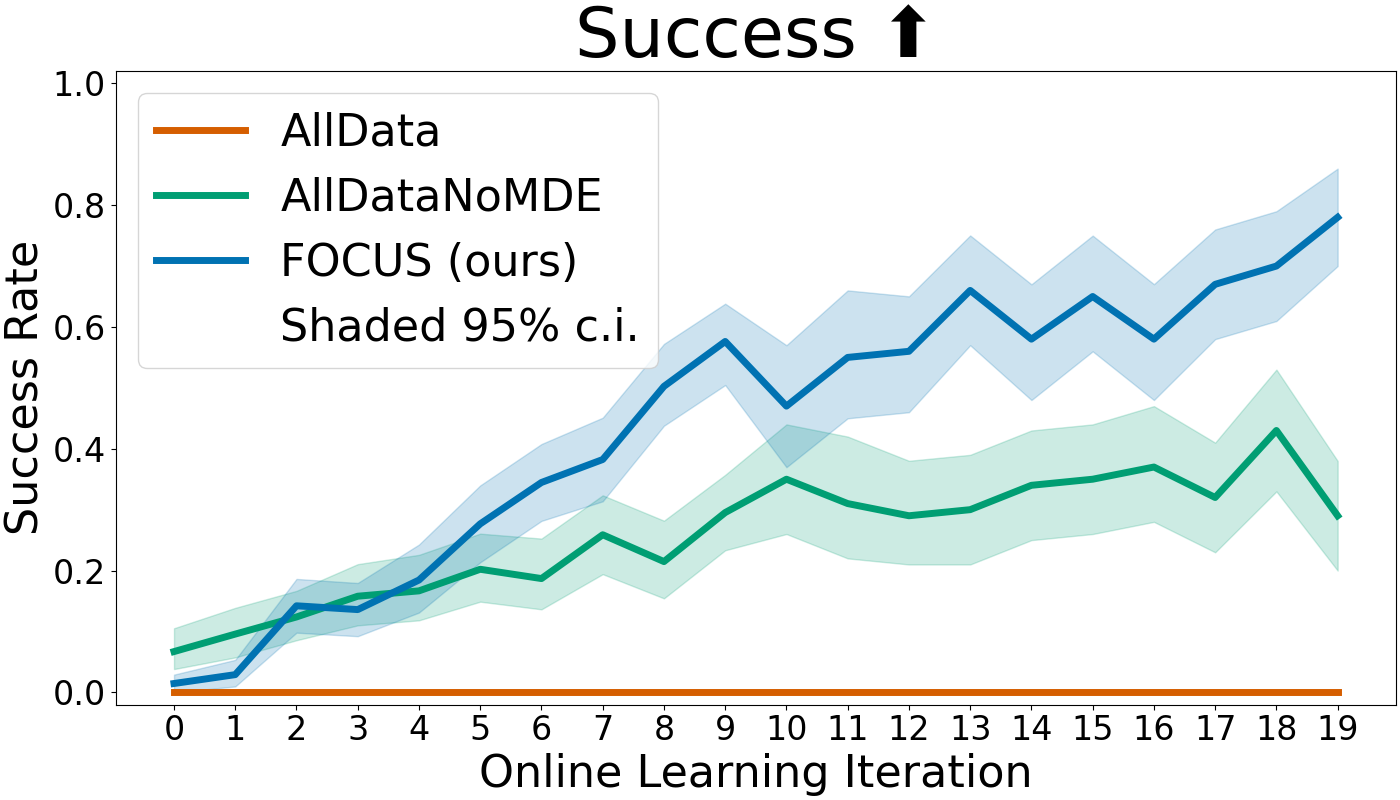
\includegraphics[width=\linewidth]{Chap4/images/success.png}
     \end{subfigure}
     \hfill
     \begin{subfigure}[b]{0.32\textwidth}
         \centering
         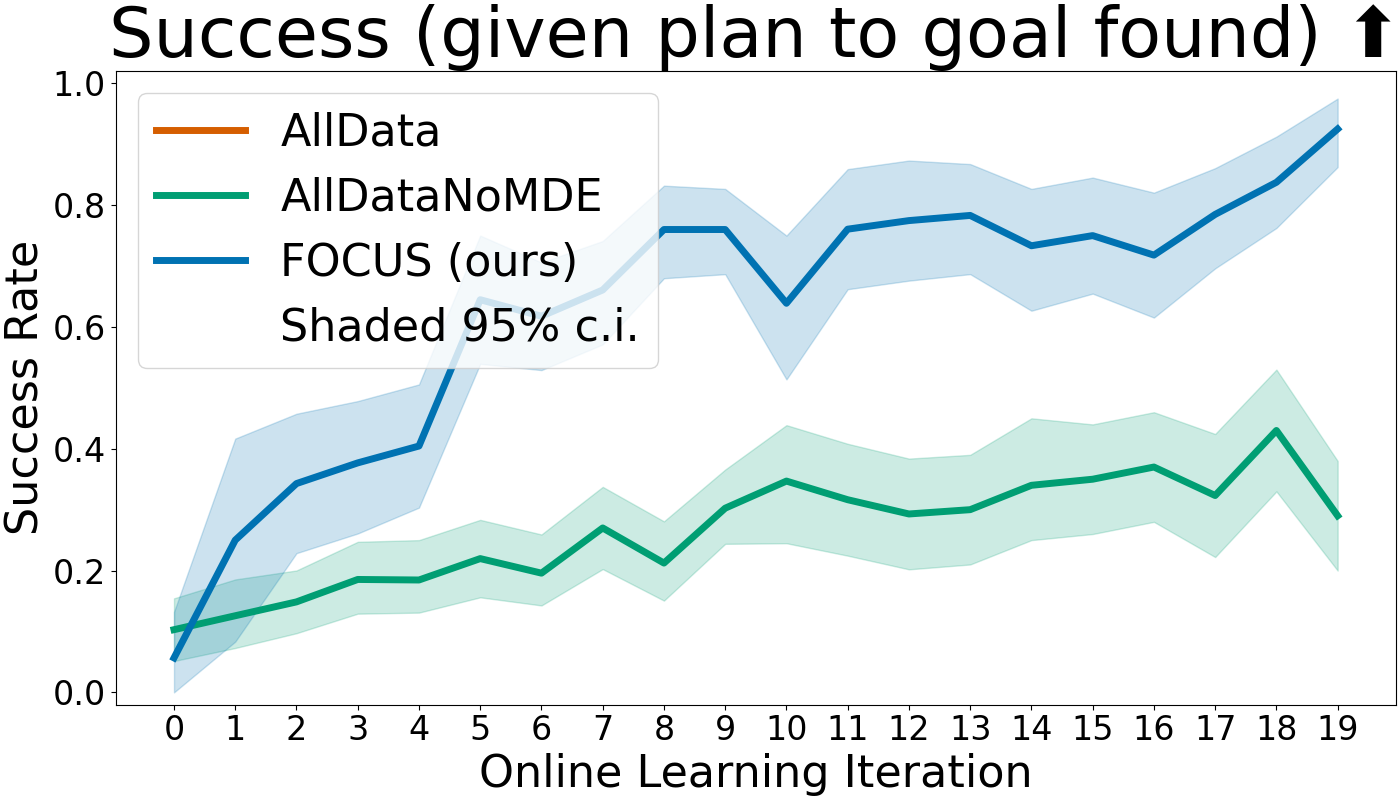
\includegraphics[width=\linewidth]{Chap4/images/success_given_plan_found.png} 
     \end{subfigure}
     \hfill
     \begin{subfigure}[b]{0.32\textwidth}
         \centering
         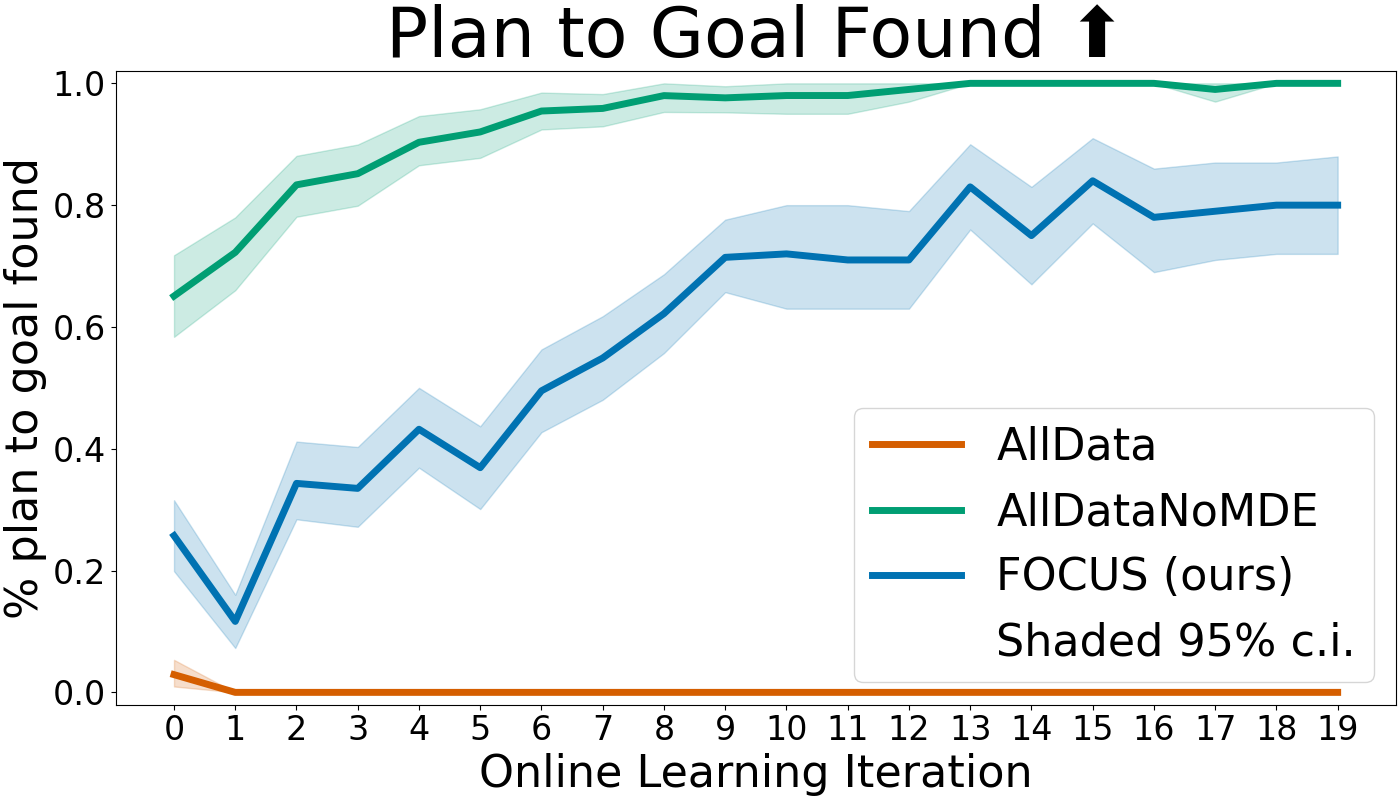
\includegraphics[width=\linewidth]{Chap4/images/plan_found.png}
     \end{subfigure}
    \caption{Post-learning evaluation of rope manipulation in simulation: Three metrics shown over the 20 iterations of online learning. The shaded interval is the 95\% confidence interval, with the boot-strapping method used by Seaborn.}
    \label{ICRA:fig:sim_rope_results}
\end{figure*}

We show that \FOCUS{} achieves higher task success with fewer data than baselines which fine-tune the dynamics on all available data. The first baseline, called \textit{AllDataNoMDE} does not use our proposed adaptation method and does not use MDEs when planning, which makes it a conventional online learning method. The second, called \textit{AllData} includes MDEs in planning, but ablates our fine-tuning method. First, we evaluate in the rope manipulation domain on adaptation from one simulation to another (see Figure \ref{ICRA:fig:sim_rope_envs}). We ran 20 iterations of online learning, where each iteration consists of 10 episodes, which amounts to roughly $6,000$ transitions in total during learning. We then repeated this 10 times for each method/baseline with different random seeds.

After learning, we took the models saved after each learning iteration and ran 100 episodes of evaluation per method. To maximize success rates of all methods, we use a longer timeout and do not allow random-accepts when planning. We also stop execution and replan if the error between the plan and the observed state exceeds a large threshold on model error (0.25).

The results of this first experiment are summarized in Figure \ref{ICRA:fig:sim_rope_results}. The proposed method (\FOCUS{}) shows the highest success rate when plans are found. The \textit{AllData} method, which ablates our method for fine-tuning the dynamics, never finds paths to the goal. This is because its dynamics are not sufficiently accurate, and so the MDE constraint makes the planning problem infeasible. Accurately learning the dynamics in the \textit{AllData} or \textit{AllDataNoMDE} methods would involve predicting the deformation of the rope on obstacles, which is challenging given a dataset of only a few thousand transitions.

\begin{figure}
    \centering
    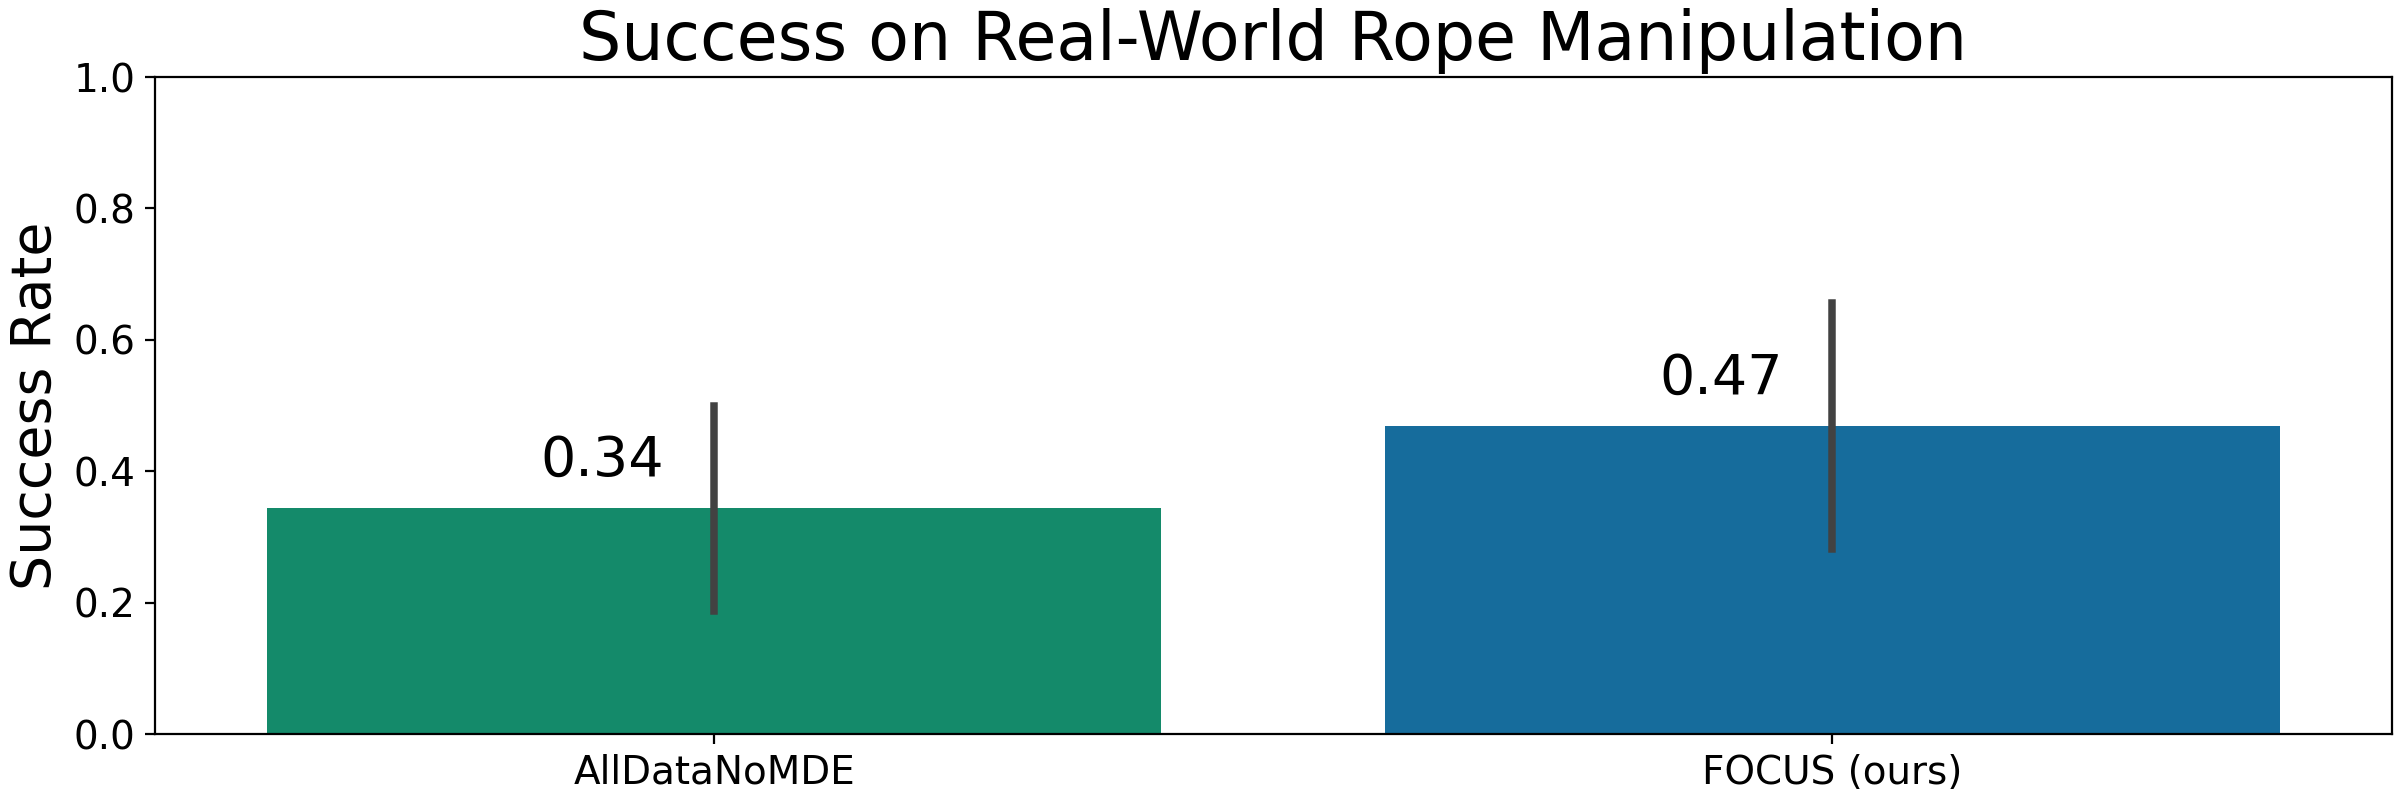
\includegraphics[width=0.7\linewidth]{Chap4/images/real_success.png}
    \caption{Success rate for the \textit{AllDataNoMDE} baseline (left) versus \FOCUS{} (right) for online adaptation to real world bimanual rope manipulation.}
    \label{ICRA:fig:real_rope_success}
\end{figure}

\subsection{Real Robot Results}

We performed a similar experiment to the first rope manipulation experiment, but on real robot hardware where sensor and actuator noise are substantial factors (approximately \SI{5}{\centi\meter} of end-effector error). More importantly, it demonstrates how \FOCUS{} enables a robot to quickly learn a task in the real world. We use CDCPD2 \cite{CDCPD2} to track the rope state. The geometry of the car scene is approximated with primitive geometric shapes. We use the same source simulation environment as for the  simulation rope experiment, but now the target environment is the real world. The robot must learn to adapt the simulated free-space rope dynamics to the real world, despite the different real-world free-space dynamics and the fact that the rope can deform on the robots' arms or on the objects in the scene. Because perception and actuation error are higher in the real world than in simulation, we use $\softFilteringThrehsold=0.2$.

We ran the online learning procedure with a single start configuration and a single goal region for one random seed and compare \FOCUS{} to the \textit{AllDataNoMDE} baseline, since \textit{AllDataNoMDE} performed best in simulation. After 15 iterations of learning, we freeze the models and evaluate task success 32 times. The success rates are shown in Figure \ref{ICRA:fig:real_rope_success}. With \FOCUS{}, the robot successfully placed the rope under the engine 15/32 times, while \textit{AllDataNoMDE} succeeded 11/32 times. Achieving high success rates in this task is difficult due to narrow passages, perception error, and actuator error. Failure modes for FOCUS include the rope getting pulled out of the robots' hands, getting too close and catching on obstacles, and failing to find plans that reach the goal.

\section{Conclusion} \label{ICRA:sec:conclusion}

This paper studies the problem of adapting learned dynamics models to datasets which contains transitions where the dynamics are very different from the source environment. This type of domain mismatch is common in online dynamics learning settings, where the source dynamics are learned in simulation or on a simpler task. Traditional adaptation methods can fail in this setting because trying to fit data from regions of dissimilar dynamics leads to poor predictions even in regions where the source and target dynamics are similar.

Our key insight is to instead focus adaptation on regions where the source and target dynamics are similar. We propose an adaptation method which assigns high weight to transitions with low prediction error, and dynamically re-assigns weights during the course of training. The set of low-error transitions is initially a small set, but grows as training pulls down the prediction error for other similar transitions. We combine our adaptation method with prior work on planning with unreliable dynamics to make \FOCUS{}, a data-efficient online adaptation method. We demonstrate that \FOCUS{} can learn a bimanual rope manipulation task in simulation and in the real world, and achieves higher task success rates than baselines which attempt to fit all the training data.
